\documentclass[a4paper, 12pt, notitlepage]{report}
\usepackage{amsmath,amsthm,amsfonts,amssymb,amscd}
\usepackage[margin=3cm]{geometry}
\usepackage{graphicx}
\usepackage{caption}
\usepackage{hyperref}
\usepackage{float}
\usepackage{subcaption}
\usepackage{esvect}
\usepackage[table,xcdraw]{xcolor}
\setlength{\parindent}{0.0in}
\setlength{\parskip}{0.05in}
\DeclareGraphicsExtensions{.pdf,.png,.jpg}

\title{Combining Multiple Evidence from Different Types of Thesaurus for Query Expansion}
\author{Sneha Shankar Narayan}
\date{\today}

\begin{document}
\maketitle
\begin{center}
\Large{
\textbf{CS646} - Information Retrieval}
\end{center}
\newpage

\tableofcontents

\chapter{Background}
Query expansion (QE) is the process of reformulating a seed query to improve retrieval performance in information retrieval operations. \cite{wiki} The given input is evaluated and additional search terms are added to in order to retrieve more relevant documents.

The approach being explored in this project is combining different types of thesaurus for query expansion. Thesauri
have frequently been incorporated in information retrieval systems as a device for the recognition of synonymous expressions and linguistic entities that are semantically similar but superficially distinct. \cite{paper}
This is based off of the idea presented in the paper "Combining multiple evidence from different types of Thesaurus for query expansion" by Rila Mandala, Takenobu Tokunaga, Hozumi Tanaka \cite{paper}. 

The basic idea is to get "related" terms to the query terms from the different thesauri individually and combining them and evaluate how the expanded queries perform as opposed to the original queries.

The various thesauri being used in this project are:
\subsection*{Wordnet based thesaurus}
WordNet is a hand-crafted thesaurus developed by Princeton University. In WordNet, words are organized into taxonomies where each node is a set of synonyms (a synset) representing a single sense. There are four different taxonomies based on different parts of speech and also there are many relationships defined among
them. \cite{paper} The paper uses the noun taxonomy only.

The similarity between words a and b can be defined as the shortest path from each sense of a to each sense of b
\begin{equation*}
sim_{path}(a, b) = max[-\log(\frac{N_p}{2D})]
\end{equation*}

where $N_p$ is the maximum number of nodes in path $p$ from a to b and $D$ is the maximum depth of the taxonomy.

\subsection*{Co-occurence based thesaurus}
This method is based on the assumption that a pair of words that occur frequently together in the same document are related to the same subject. Therefore word co-occurrence information can be used to identify semantic relationships between words.\cite{paper}

The text is subdivided into pseudo-sentences of word-size 3, and each word in the query is compared against the words in the documents to determine co-occurrence. Mutual-information is used as a tool for computing similarity between words. Mutual information compares the probability of the co-occurrence of words a and b with the independent probabilities of occurrence of a and b:

\begin{equation*}
I(a,b) = \log\frac{P(a,b)}{P(a)P(b)}
\end{equation*}

where the probabilities of $P(a)$ and $P(b)$ are estimated by counting the number of occurrences of a and b in the document. The joint probability is estimated by counting the number of times that word a co-occurs with b

\subsection*{Combined approach}
The similarities from the above two approaches are averaged to calculate the similarities between two words a and b in the combined approach

\begin{equation*}
sim_{combined} (a,b) = \frac{sim_{wordnet} + sim_{co-occurence}}{2}
\end{equation*}

Since the similarities can be of an range they are normalized before being plugged into the above formula. For all similarities that are computed in the wordnet and co-occurence approaches the following formula is applied

\begin{equation*}
sim_{new} = \frac{sim_{old} - sim_{min}}{sim_{max} - sim_{min}}
\end{equation*}


%	\paragraph
%The words having the similarity value above a certain threshold are picked and the queries are expanded. A query q %is expanded by adding the vector
%\begin{equation*}
%\vv{q} = (w_1^', w_2^',...,w_n^' )
%\end{equation*}

%Sto the original query vector. $$w_j^'$$ is equal to $$w_{ex}(q, t_j)$$ if it exceeds a certain threshold.

\chapter{Evaluation Methodology}
The original queries are expanded using the terms determined by each of the three approaches. The queries are run on Galago \cite{galago} and the new ranked lists are obtained. 

The determined ranked lists are checked against the baseline (the experiments performed as a part of P2) and the following measures of interest are obtained
\begin{itemize}
\item Average precision and Mean average precision
\item NDCG @ 10
\item Precision @ 10
\end{itemize}

The queries in the books-medium collection, the queries for the robust collection from the class, and the TRECRobust collection were used to perform the experiments.

\chapter{Implementation}
The queries that were obtained from the various collections had to be expanded and the implementation of the query expansion in each type of thesaurus was done using Python.

In order to help with the implementation, all the word-similarity computation was done with the query words and the words in the top 50 ranked documents of the original query. Thus query expansion was basically done on the fly. 

\subsection*{Wordnet based thesaurus}
The wordnet thesaurus was made available to python using textblob \cite{textblob} a text processing library for python. First, the top 50 documents were retrieved for the original query and the wordnet path similarity between every query word and the other words were computed. 

The similarity threshold of 0.5 was applied to determine the similar words and for each query word the top 3 similar words were added to the query as long as the similarity threshold was met.
 
\subsection*{Co-occurence thesaurus}
The top 50 documents for the original query was retrieved. Counters are managed for the number of occurences of each of the query words in the retrieved documents. Hashes are managed to get the most co-occuring words with the query words in the documents revtrived. Mutual information values are computed for the co-occuring words.

The similarity threshold (mutual information values) of 0.5 was applied to determine the similar words and for each query word the top 2 similar words were added to the query as long as the similarity threshold was met.  

\subsection*{Combined approach}
The similarities obtained from the above two methods were averaged and the set of words that were determined from both the approaches were added to the original query in order to expand it.

\subsection*{Process}
The query expansion and evaluation on each of the approaches had the following steps
\begin{enumerate}
\item Parse the queries.xml file in all the datasets and send each query to the script (of the method being evaluated) which does the query expansion.
\item The obtained query along with the query number which is got from the XML file is output to a json file.
\item Run the expanded queries on Galago and get the ranked list.
\item Evaluate the expanded queries against the relevance judgements using the evaluation scripts that were written for P2.
\end{enumerate}


\chapter{Results and Analysis}

The evaluation measures computed are the following:

\subsection*{Mean average precision}

% Please add the following required packages to your document preamble:
% \usepackage[table,xcdraw]{xcolor}
% If you use beamer only pass "xcolor=table" option, i.e. \documentclass[xcolor=table]{beamer}
\begin{table}[h]
\begin{tabular}{| p{2.5cm} | p{2.5cm} | p{2.5cm} | p{2.5cm} | p{2.5cm} |}
\hline
\rowcolor[HTML]{BBDAFF} 
                                         & Baseline (P2) & Wordnet Thesaurus & Co-occurence Thesaurus & Combined Approach \\ \hline
\cellcolor[HTML]{BBDAFF}Books            & 0.3647        & 0.1954 (-46\%)    & 0.2906(-20.3\%)        & 0.2047 (-43.84\%) \\ \hline
\cellcolor[HTML]{BBDAFF}Robust-class     & 0.3910        & 0.2812 (-28\%)    & 0.3811 (-2 \%)         & 0.2879 (-26.3\%)  \\ \hline
\cellcolor[HTML]{BBDAFF}Robust-community & 0.2295        & 0.1549 (-32\%)    & 0.1843 (-19.69 \%)     & 0.1582 (-31.06\%) \\ \hline
\end{tabular}
\end{table}

\subsection*{Graphs}
For easier analysis of the obtained results, it's interesting to see how the average precision works across the data sets:

Average precision on the books-medium queries:
\begin{center}
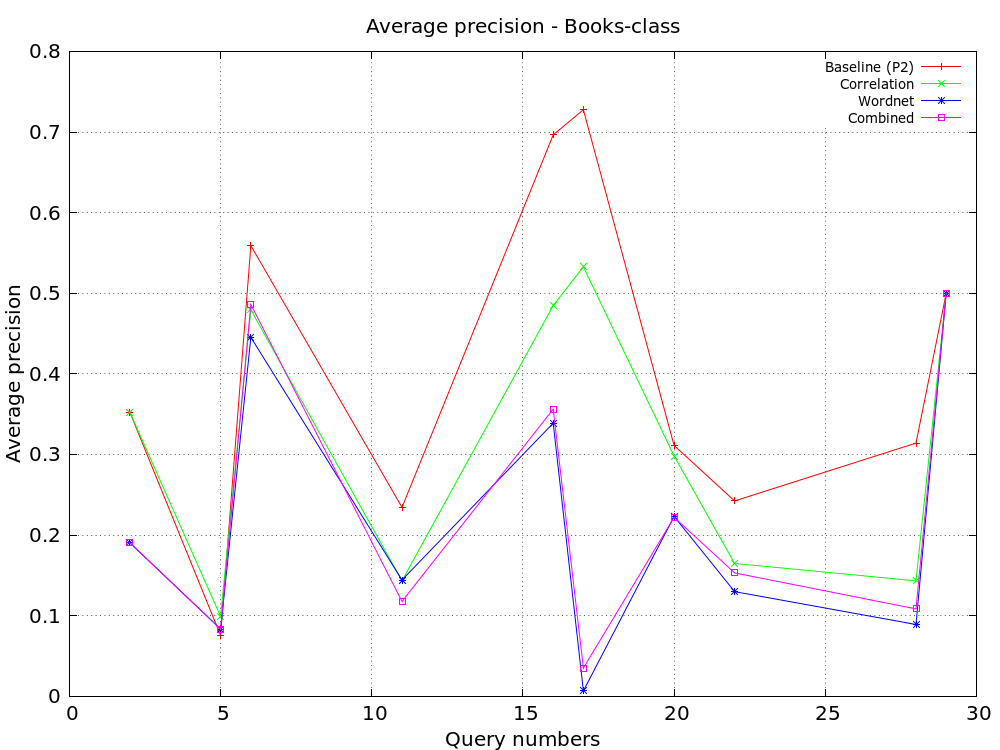
\includegraphics[scale = 0.4]{books_avg}
\end{center}

Average precision on the robust queries from class:
\begin{center}
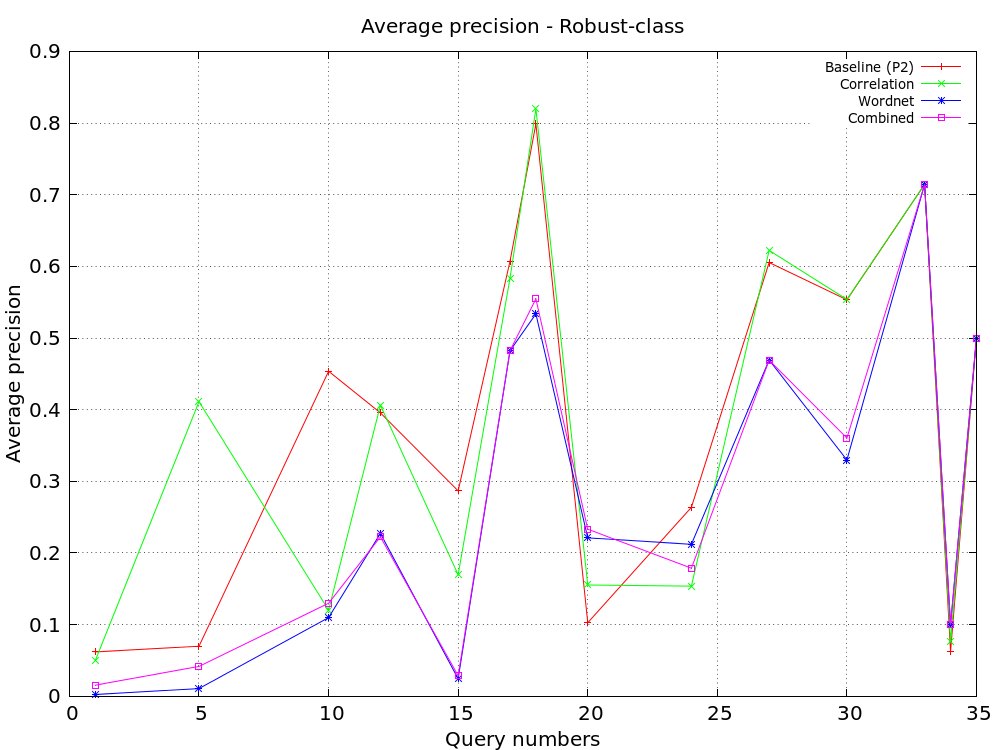
\includegraphics[scale = 0.4]{robust-class_avg}
\end{center}

Average precision on the robust04 queries:
\begin{center}
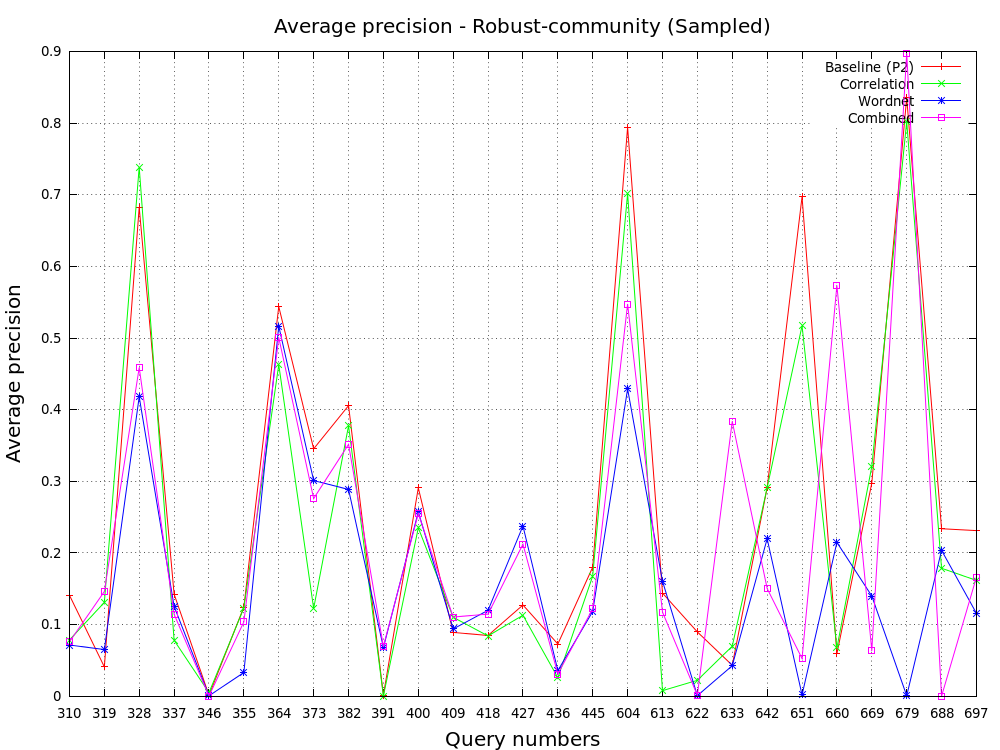
\includegraphics[scale = 0.4]{sampled-robust-comm_avg}
\end{center}

From the above plots valid conclusions can be drawn from the robust04 query results. We notice that the graphs for co-occurence based thesaurus queries and the 


\chapter{Conclusion}

Though in theory thesaurus 

\begin{thebibliography}{1}
\bibitem{wiki} \url{http://en.wikipedia.org/wiki/Query_expansion}
\bibitem{paper} \url{http://www.iro.umontreal.ca/~nie/IFT6255/mandala99combining.pdf}
\bibitem{textblob} \url{http://textblob.readthedocs.org/en/dev/}
\end{thebibliography}



\end{document}